\documentclass[12pt,a4paper]{ctexart}  
\usepackage[utf8]{inputenc}
\usepackage{easyReview}
\usepackage[T1]{fontenc}
\usepackage{amsmath}
\usepackage{fancyhdr}  %设置论文的页眉页脚
\usepackage{amsfonts}
\usepackage{multirow}
\usepackage{booktabs}
\usepackage{amssymb}
\usepackage{amsmath}
\usepackage{multirow}   %???
\usepackage{booktabs}
\usepackage{subcaption}
\usepackage{float}
\usepackage{amsfonts}
\usepackage{mathrsfs}
\usepackage{amssymb}
\usepackage{mathrsfs}
\usepackage{bm}
\usepackage{extarrows}  %等号上面加文字
\usepackage{extarrows}
\usepackage{wasysym}   %添加表情
\usepackage{graphbox}  %图片放右侧
\usepackage{graphicx}
%\usepackage{subfig}
%\usepackage{subfloat}
\usepackage[colorlinks,linkcolor=red,anchorcolor=blue,citecolor=green]{hyperref}
\usepackage{amssymb}
\usepackage{mathrsfs}
\usepackage{cases}   %多个公式一起编号
\usepackage{color}
\usepackage{tcolorbox}
\usepackage{listings}
\usepackage{xcolor}
\usepackage[framemethod=tikz]{mdframed}  %高亮显示某段文字
\usepackage[left=2.00cm, right=2.00cm, top=2.00cm, bottom=2.00cm]{geometry}

\newcommand{\RNum}[1]{\uppercase\expandafter{\romannumeral #1\relax}}        %添加罗马数字
\newtheorem{theorem}{定理}[section] % 定义一个定理环境，名为定理，编号依赖于 section
\newtheorem{lemma}[theorem]{Lemma} % 定义一个引理环境，名为引理，编号与定理共用
\newtheorem{definition}[theorem]{定义}
\newtheorem{example}[theorem]{例}
\newtheorem{exercise}[theorem]{\textcolor{blue} {练习}}
\newtheorem{problem}[theorem]{问题}
\newtheorem{property}[theorem]{性质}
\newtheorem{proposition}[theorem]{命题}
\newtheorem{remark}[theorem]{Remark}
\newtheorem{algorithm}[theorem]{算法}
\pagestyle{fancy}  %定义页码，页眉，页脚
\cfoot{\thepage}  %去掉页脚中间部分
\lhead{{《最优化理论与方法》实验报告}}


\begin{document}


% 我们开始自定义封面，首先设置封面不显示页号
% \pagestyle{empty}
% 来一个无法拒绝的垂直间距，大约是 12 个 M 字符的长度
\vspace*{6em}

\begin{figure}[H]
	\centering
	
\includegraphics[width=0.4\linewidth]{picture/HNUlogo}
\end{figure}
\vspace*{4em}
% 标题
\begin{center}
{\Huge \bf 《最优化算法与理论》 实验报告}  %\bigskip  % 垂直间距
\end{center}
\vspace{4em}  % 垂直间距
% 信息
\begin{center}
{\Large  % 这里的字号也可以用别的方式修改

{\bf\makebox[4em][s]{实验序号}}: \underline{\makebox[13em][c]{1}}\\
{\bf\makebox[4em][s]{实验内容}}: \underline{\makebox[13em][c]{线性搜索法}}\\
{\bf\makebox[4em][s]{班~~~~级}}: \underline{\makebox[13em][c]{信息2301}}\\
{\bf\makebox[4em][s]{学~~~~号}}: \underline{\makebox[13em][c]{202310040128}}\\
{\bf\makebox[4em][s]{姓~~~~名}}: \underline{\makebox[13em][c]{雷龙浩}}\\
{\bf\makebox[4em][s]{完成日期}}: \underline{\makebox[13em][c]{2026年03月21日}}\\

}
\end{center}
\clearpage

\newpage

\tableofcontents
\newpage


\section{实验概述与分析}

\subsection{实验目标与问题描述}
本实验旨在研究非线性优化中的线搜索（Line Search）策略。针对目标函数 $f(x) = (x_1 - x_2)^2 + x_2^2$，
在给定点 $x_0$ 和方向 $d_0$ 下，对比三种不同性质的步长确定方法：
\begin{itemize}
	\item 精确搜索：黄金分割法（求取使函数值最小的绝对最优步长）。
	\item 非精确搜索（充分下降）：Armijo 准则（保证函数值下降，计算开销小）。
	\item 非精确搜索（高效下降）：Wolfe-Powell 准则（兼顾下降量与梯度变化，保证算法稳定性）。
\end{itemize}

\subsection{算法原理与实现逻辑描述}
\subsubsection{黄金分割法：}
\begin{itemize}
	\item 该算法通过\textbf{缩小区间}的策略(类似于二分法)寻找一元函数 $\phi(\alpha)$ 的极小点。
	\item 它利用黄金分割比例 $\tau \approx 0.618$ 在初始区间内取测试点。
	\item 逻辑核心：每次迭代比较两个测试点的函数值，剔除较大点以压缩搜索区间，直到区间长度小于设定的精度 $\epsilon$。
	\item 特点：不依赖导数信息，但对初始区间的选择较为敏感。对于单峰函数可以稳定收敛到最优。
\end{itemize}

\subsubsection{Armijo 型线搜索描述：}
\begin{itemize}
	\item 这是一种典型的回溯算法，旨在寻找一个满足“充分下降”条件的步长。
	\item 充分下降条件：$f(x_k + \alpha d_k) \leq f(x_k) + \sigma_1 \alpha \nabla f(x_k)^T d_k$。
	\item 实现逻辑：从一个初始大步长开始，如果不满足条件，则说明步长太大了，通过因子 $\rho$ 不断衰减 $\alpha$，
			直到步长落入由 $\sigma_1$ 确定的斜率控制线之下。
	\item 缺点：Armijo 条件只能保证步长不过大，但不能保证步长不过小。
\end{itemize}

\subsubsection{Wolfe-Powell 型线搜索描述：}
\begin{itemize}
	\item 在 Armijo 条件的基础上增加了曲率条件，防止步长过小导致迭代效率低下。
	\item 双重约束：既要满足函数值显著下降（充分下降条件），又要保证新点处的坡度变平缓（曲率条件）。
	\item 曲率条件：$ \nabla f(x_k + \alpha_k d_k)^T d_k \geq \sigma_2 \nabla f(x_k)^T d_k $
	\item 实现逻辑：采用“回溯+外推”的组合手段。先找到满足下降条件的区间，再通过类似插值的方式在其中搜寻满足曲率要求的高质量步长。
\end{itemize}


我们用 Python 编写程序实现了黄金分割法{\color {blue} （程序见作业附件压缩文件包）}. 程序代码主体如下：
\begin{figure}[H]
	\centering
	
\includegraphics[width=\linewidth]{picture/1}
	\caption{黄金分割法程序.}
\end{figure}

\subsection{算法程序实现}
我们用 Python 编写程序实现了Armijo 型线搜索法{\color {blue} （程序见作业附件压缩文件包）}. 程序代码主体如下：
\begin{figure}[H]
	\centering
	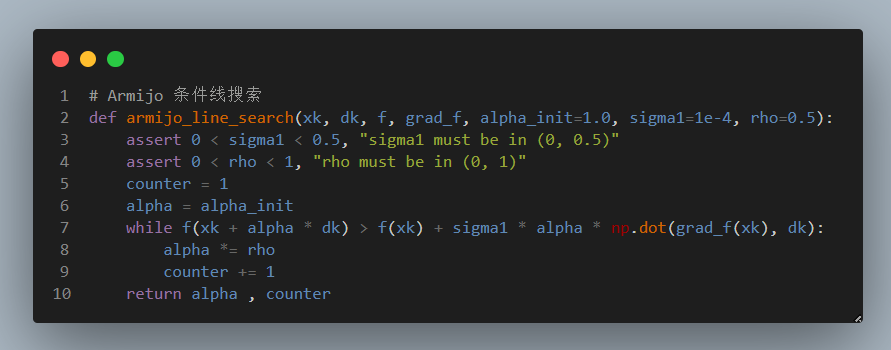
\includegraphics[width=0.9\linewidth]{picture/2}
	\caption{Armijo 型线搜索法.}
\end{figure}


我们用 Python 编写程序实现了Wolfe-Powell 型线搜索{\color {blue} （程序见作业附件压缩文件包）}. 程序代码主体如下：
\begin{figure}[H]
	\centering
	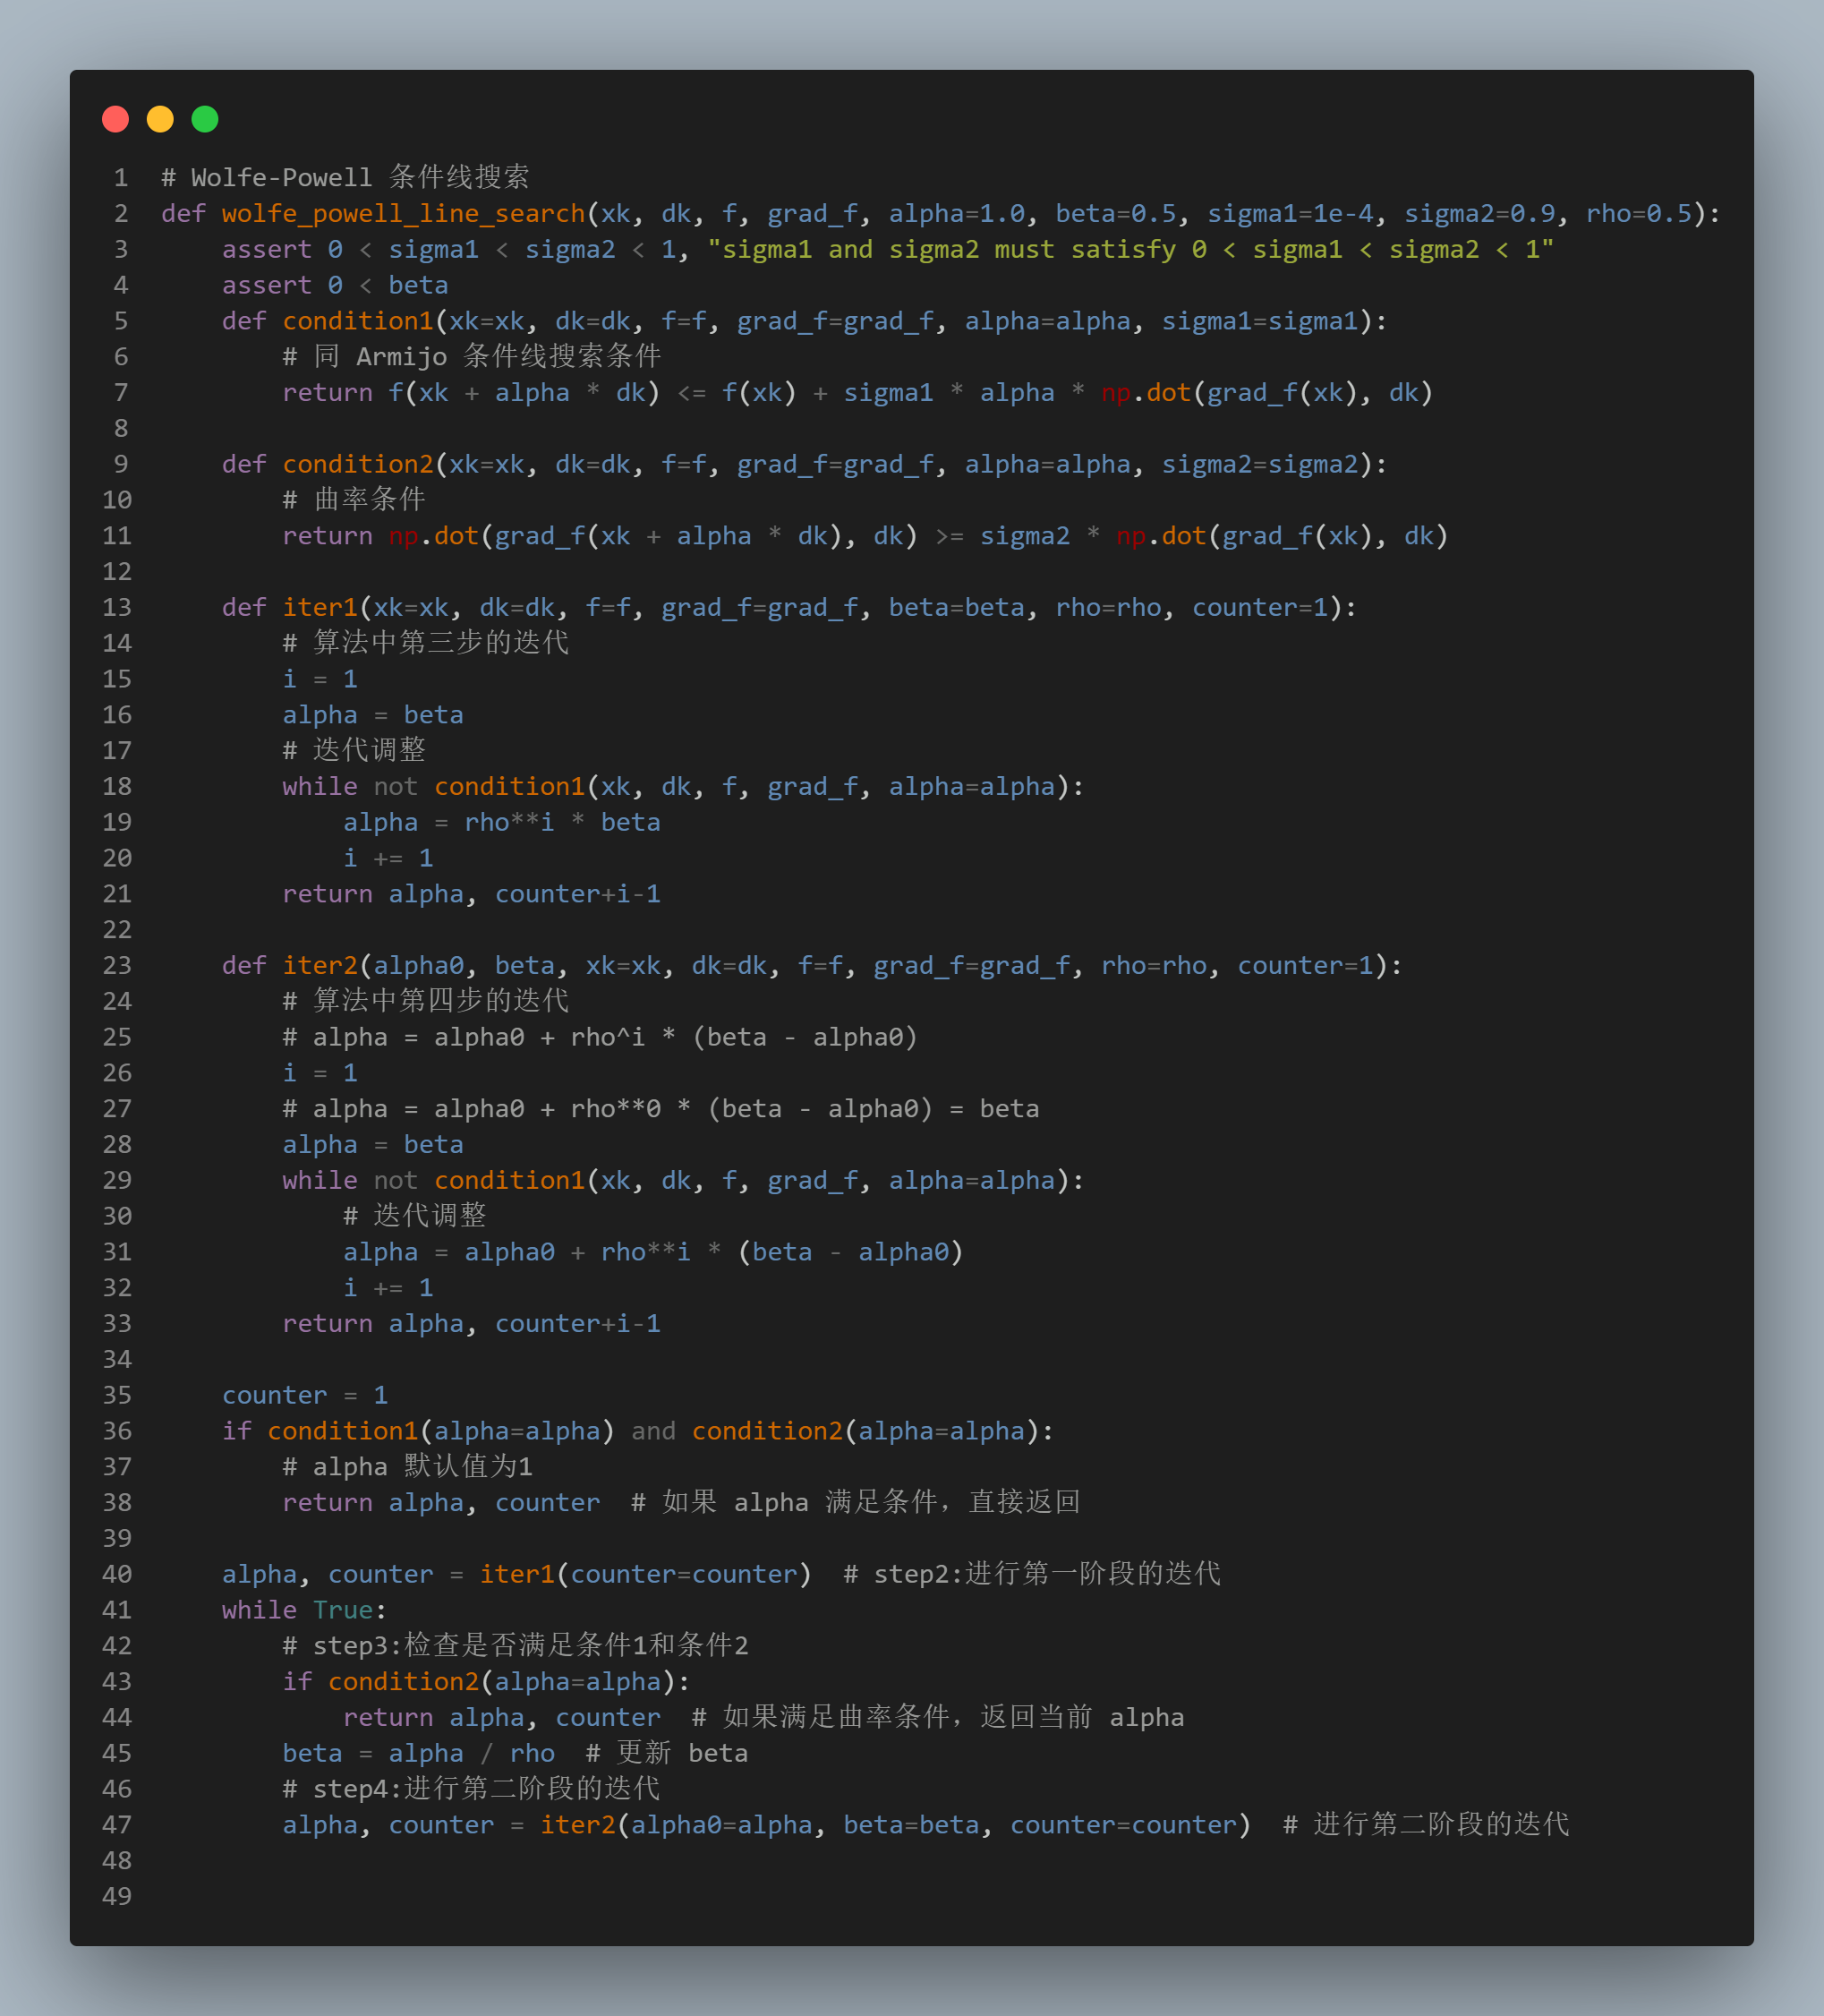
\includegraphics[width=\linewidth]{picture/3}
	\caption{Wolfe-Powell 型线搜索法.}
\end{figure}




\section{固定方向 $d_0$ 的三种方法运行结果及参数敏感性分析}
\subsection{理论分析}
\begin{quotation}
	计算函数 $f(x) = (x_1 - x_2)^2 + x_2^2$ 在点 $x_0 = (0, 1)^T$ 处，
	沿着方向 $d_0 = -(1, 1)^T = (-1, -1)^T$ 的精确步长 $\alpha$。
\end{quotation}

对于黄金分割法，我们的目标是构造一元函数 $\phi(\alpha)$
$\alpha > 0$，使得 $\phi(\alpha) = f(x_0 + \alpha d_0)$ 最小。\\
对于该题，确定位置向量：
$$x_0 + \alpha d_0 = \begin{pmatrix} 0 \\ 1 \end{pmatrix} + \alpha \begin{pmatrix} -1 \\ -1 \end{pmatrix} = \begin{pmatrix} -\alpha \\ 1 - \alpha \end{pmatrix}$$
代入原函数 $f(x)$：$$\begin{aligned} \phi(\alpha) &= f(-\alpha, 1-\alpha) \\ &= [-\alpha - (1 - \alpha)]^2 + (1 - \alpha)^2 \\ &= (-1)^2 + (1 - \alpha)^2 \\ &= 1 + (1 - \alpha)^2 \end{aligned}$$
显然，这是一个关于 $\alpha$ 的二次函数，其极小值点在 $\alpha = 1$ 处。
故在黄金分割法中，我们可以选取区间迭代$[0,2]$来逼近最优步长$\alpha = 1$ 。


\subsection{实验结果统计}

\begin{table}[H]
\centering
\caption{固定起点 x0 和固定方向 d0 的线搜索求步长，参数敏感性分析}
\begin{tabular}{cccc}
\toprule
\textbf{Method}          & \textbf{Parameter}          & \textbf{Alpha}      & \textbf{Iters} \\
\midrule
GoldenRatio     & $eps=0.01$           & 1.000020   & 13   \\
GoldenRatio     & $eps=0.0001$         & 1.000020   & 22   \\
GoldenRatio     & $eps=1e-06 $         & 1.000000   & 32   \\
\midrule
Armijo          & $sigma1=0.0001 $     & 1.250000   & 3    \\
Armijo          &$ sigma1=0.1 $        & 1.250000   & 3    \\
Armijo          & $sigma1=0.2  $       & 1.250000   & 3    \\
Armijo          & $rho=0.2$         & 1.000000   & 2    \\
Armijo          & $rho=0.5 $        & 1.250000   & 3    \\
Armijo          &$ rho=0.8$         & 1.638400   & 6    \\
\midrule
Wolfe           & $sigma2=0.1 $          & 1.000000   & 1    \\
Wolfe           & $sigma2=0.5 $          & 0.500000   & 1    \\
Wolfe           & $sigma2=0.9$           & 0.500000   & 1    \\
\midrule
Wolfe           & $beta=0.1 $            & 0.100000   & 1    \\
Wolfe           & $beta=0.5$             & 0.500000   & 1    \\
Wolfe           & $beta=2.0 $            & 1.000000   & 2    \\
Wolfe           &$ beta=5.0$             & 1.250000   & 3    \\
\bottomrule
\end{tabular}
\end{table}

\subsection{参数分析}
\begin{enumerate}
	\item 黄金分割法（精确搜索）\\
	数据表明，黄金分割法能够极其稳定地逼近理论最优解 $\alpha = 1.0$。
	随着容差 eps 从 $0.01$ 缩小至 $10^{-6}$，迭代次数（Iters）从 13 次显著增加到 32 次。
	精确线搜索具有对数级别的收敛稳定性，不依赖于目标函数的导数信息。
	但在要求高精度（$10^{-6}$）时，大量的内部函数估值迭代会导致极大的计算开销。

	\item Armijo 准则（回溯型非精确搜索）\\
	\textbf{（注：从前面的分析可知最优步长为，$\alpha_{init} = 1.0$
	以下实验采用了较大的初始尝试步长， $\alpha_{init} = 5.0$ 以触发回溯）}\\
	\begin{itemize}
		\item \textbf{对 $\sigma_1$（充分下降系数）的敏感性较低：}当 $\sigma_1$ 在 $0.0001$ 到 $0.2$ 之间变化时，
		最终求得的步长（$1.25$）和迭代次数（$3$ 次）完全没有变化。
		这说明对于当前平滑的二次函数，只要初始步长进入了下降区域，
		绝大多数合理的 $\sigma_1$ 都能轻易被满足，算法对该参数具有很强的鲁棒性。
		\item \textbf{对 $\rho$（步长衰减因子）的敏感性较高：}当 $\rho = 0.8$（衰减慢）时，步长在回溯中缩减得很精细，
		最终停在 $\alpha = 1.6384$（$5.0 \times 0.8^4 \approx 2.048$，再乘 $0.8$ 为 $1.6384$）。
		虽然满足了下降条件，但这导致了最多的迭代次数（6 次），且步长距离最优解 $1.0$ 较远。
		当 $\rho = 0.2$ 时 $5.0 \times 0.2 = 1.0$，恰好命中了极小值点。
		因此，$\rho$ 决定了搜索网格的粗细。$\rho$ 越大，搜索越细致但开销越大；$\rho$ 越小，
		速度越快但容易错过优质解。工程上通常取 $\rho = 0.5$（二分搜索）作为折中。
	\end{itemize}

	\item \textbf{Wolfe-Powell 准则（双重条件搜索} \\
	\begin{itemize}
		\item \textbf{对 $\sigma_2$（曲率条件系数）的敏感性：}
		当 $\sigma_2 = 0.1$ 时（条件严苛，要求坡度极度平缓），算法输出了极其精确的最优解
		$\alpha = 1.0$。当 $\sigma_2 = 0.5$ 或 $0.9$ 时（条件宽松），算法接受了次优解 $\alpha = 0.5$。
		由此看出$\sigma_2$ 直接控制了非精确搜索逼近精确搜索的程度。$\sigma_2$ 越小，求得的步长越精确。
		\item \textbf{对 $\beta$（回溯系数）的敏感性：}
		当 $\beta$ 较小（$0.1, 0.5$）时，算法极易在 1 次迭代内满足条件，但得到的步长偏短（$0.1$）。
		当 $\beta$ 较大（$2.0, 5.0$）时，算法有更大的空间通过回溯（乘以 $\rho$）寻找更长、更优质的步长
		（最终得到了 $1.0$ 和 $1.25$更接近$1$），但内部迭代次数增加至 2-3 次。
	\end{itemize}
	
\end{enumerate}




\section{最速下降法的三种方法运行结果及参数敏感性分析 }

\subsection{最速下降法代码展示}
\begin{figure}[H]
	\centering
	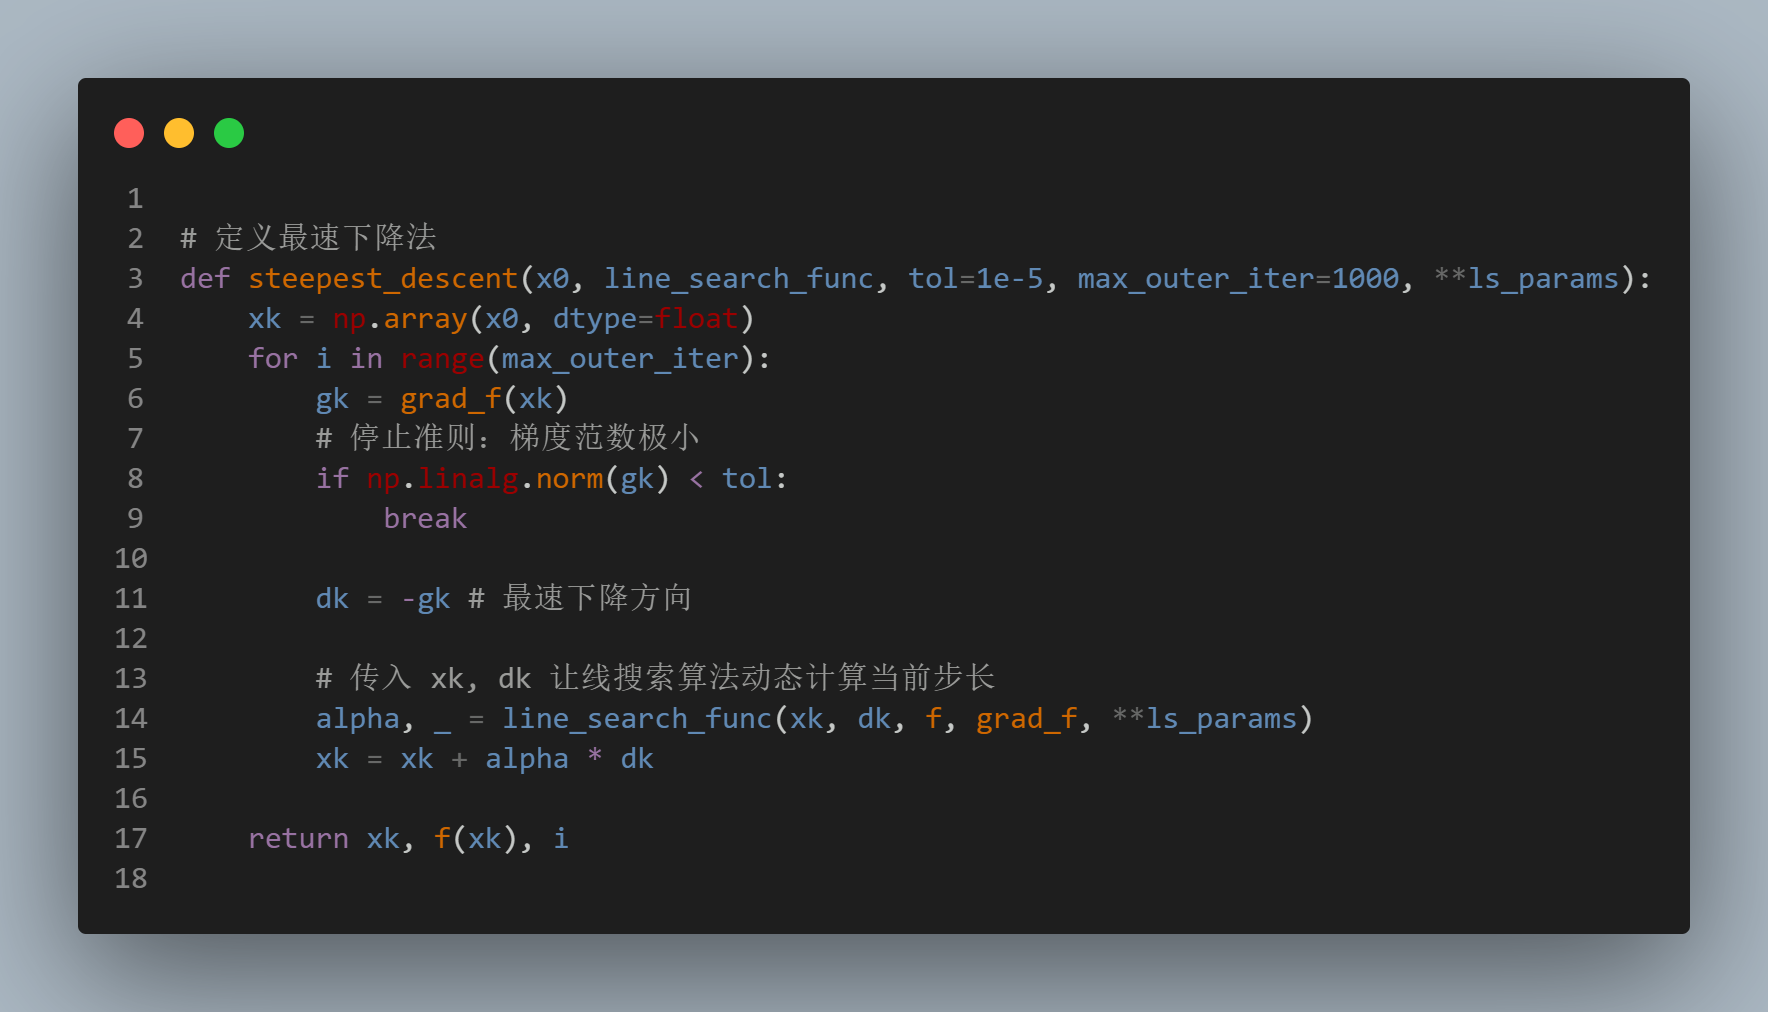
\includegraphics[width=\linewidth]{picture/4}
	\caption{最速下降法.}
\end{figure}


\begin{table}[htbp]
    \centering
    \caption{最速下降法的三种方法运行结果}
    \vspace{0.2cm}
    \begin{tabular}{llcc}
        \toprule
        \textbf{Method} & \textbf{Parameter} & \textbf{ Opt Value $f(x^*)$} & \textbf{ SD Iters} \\
        \midrule
        SD + Golden &  $\epsilon = 10^{-4}$ & $2.48 \times 10^{-10}$ & 7 \\
        \midrule
        SD + Armijo  &  $\rho = 0.2$  & $1.31 \times 10^{-11}$ & 15 \\
        SD + Armijo  &  $\rho = 0.5$  & $2.91 \times 10^{-11}$ & 33 \\
        SD + Armijo  &  $\rho = 0.8$  & $1.01 \times 10^{-11}$ & 42 \\
        \midrule
        SD + Wolfe-Powell &  $\sigma_2 = 0.1$ & $2.91 \times 10^{-11}$ & 33 \\
        SD + Wolfe-Powell &  $\sigma_2 = 0.5$ & $2.91 \times 10^{-11}$ & 33 \\
        SD + Wolfe-Powell &  $\sigma_2 = 0.9$ & $2.91 \times 10^{-11}$ & 33 \\
        \bottomrule
    \end{tabular}
\end{table}

\subsection{参数分析}
\begin{enumerate}
    \item \textbf{黄金分割法}
    当采用黄金分割法求解精确步长时，最速下降法仅需 7 次外层迭代即可收敛，远低于非精确搜索。
    其理论依据在于：精确搜索保证了相邻两次迭代的搜索方向严格正交（$\nabla f(x_{k+1})^T \nabla f(x_k) = 0$），
    在当前方向上取得了最大下降量。然而，这 7 步外层迭代的代价是每一次都需要在内部执行数十次的黄金分割区间收缩运算。
    
    \item \textbf{Armijo 准则}
    实验数据表明，衰减因子 $\rho$ 显著影响最速下降法的全局迭代次数（$\rho=0.8$ 时为 42 次，$\rho=0.2$ 时为 15 次）。
    其理论依据在于：对于存在狭长山谷特征的二次函数，较大的 $\rho$ 导致回溯步长衰减缓慢、单步跨度偏大，
	算法极易越过谷底到达对侧，从而加剧了最速下降法固有的\textbf{锯齿现象}，使得外层迭代次数激增。
	相反，较小的 $\rho$ 激进地缩小了搜索步长，在一定程度上抑制了越过谷底的震荡，改善了收敛轨迹。
    
    \item \textbf{Wolfe-Powell 准则}
    实验表明，在不同曲率系数 $\sigma_2 \in \{0.1, 0.5, 0.9\}$ 下，算法的外层迭代次数恒为 33 次，且与 $\rho=0.5$ 的 Armijo 准则表现完全一致。
    其理论依据在于：对于本实验中性质良好的平滑二次凸函数，算法在第一阶段（按默认 $\rho=0.5$ 回溯）
	找到的满足充分下降条件的试探步长 $\alpha_k$，其切线斜率已经足够平缓，自然满足了所有的曲率条件限制（包括最严苛的 $\sigma_2=0.1$）。
	因此，算法未触发第二阶段的扩展插值逻辑，直接退化为标准 Armijo 搜索。
	这证明 Wolfe 准则在良态区域内不产生额外计算开销，仅在劣态区域起到防止步长过短的保护作用。
\end{enumerate}


\end{document}


























